\chapter{Simulation Results}
\section{MPC}
An MPC comtoller will be used with the same purpose as LQR: to control the pendulum at the upright position. The optimization problem \ref{mpcformu;ation} is solved via using $quadprog$ solver in MATLLAB.
To design an MPC controller we have to define weight matrices $Q_x$ and $Q_u$:
\begin{equation}
Q_x = \begin{bmatrix}
1.5&0&0&0\\
0&0.08&0&0\\
0&0&10&0\\
0&0&0&0.2
\end{bmatrix} \quad Q_u = 1
\end{equation}
And set constrains for the control input:
\begin{equation}
	\begin{split}
	u_{min} = -5\\
	u_{max} = 5
	\end{split}
\end{equation}
We use the same initial condition as with the LQR
\newpage
\begin{figure}[H]
	\centering
	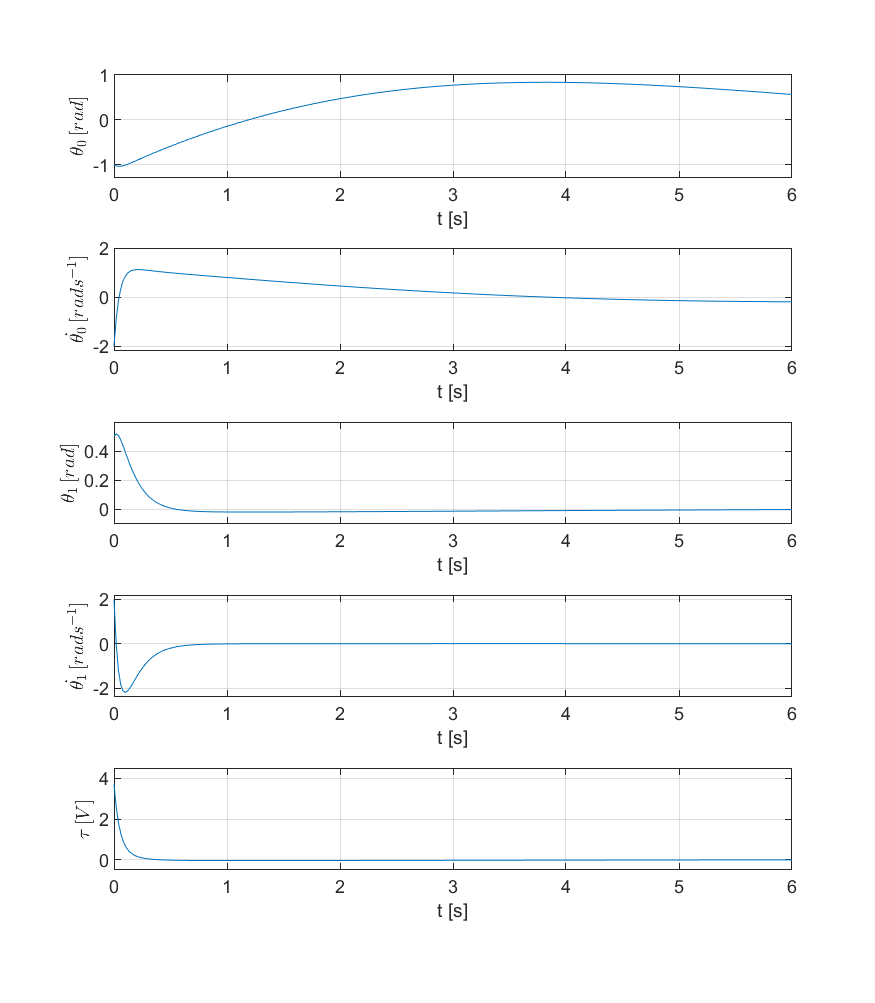
\includegraphics[width=1.1\linewidth]{images/MPC}
	\caption{Control with MPC: simulation}
	\label{mpc}
\end{figure}
\newpage
\section{Swing-Up}
The main purpose of the Swing-Up controller is to swing the pendulum from the downside position into the upright position where the control of the process will be taken by another controller.
\newpage
\begin{figure}[H]
	\centering
	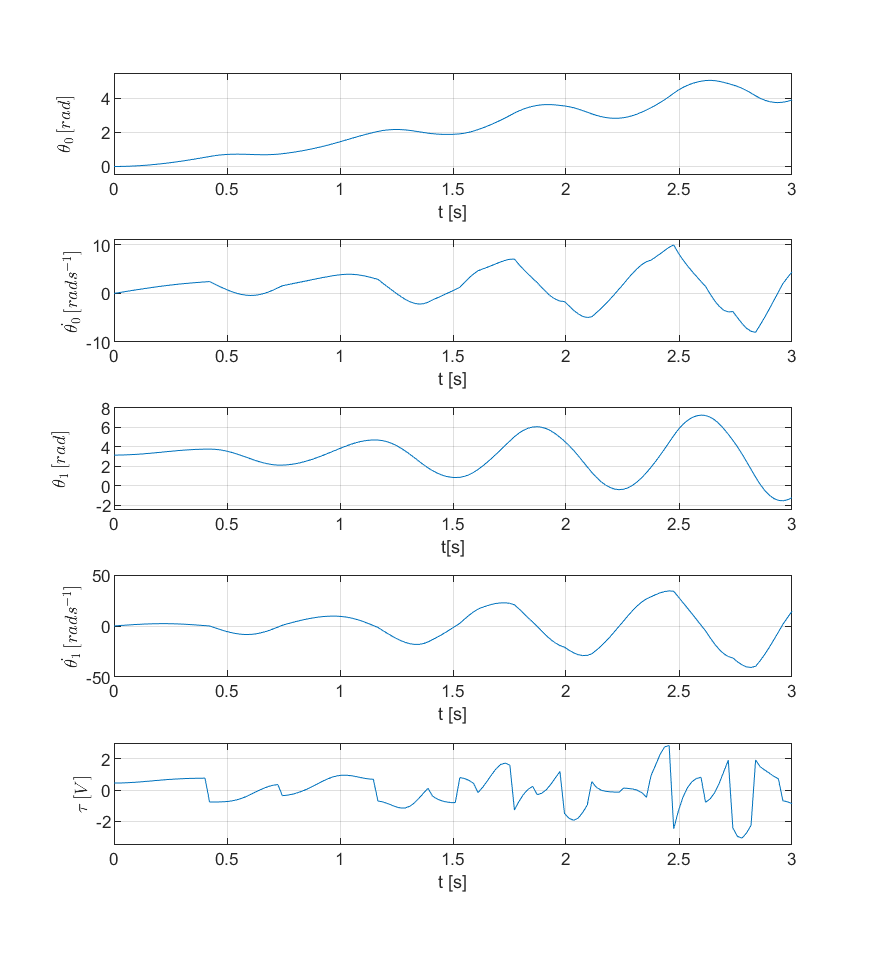
\includegraphics[width=1.1\linewidth]{images/Swing}
	\caption{Control with Swing-Up: simulation}
	\label{swing}
\end{figure}
\newpage
\section{Combined Control Strategy}
Now we combine the Swing-Up controller with an LQR or MPC controller to fully control the process. The strategy is the following: at the beginning, we oscillate the pendulum from the steady-state at the downside position with the Swing-Up controller. With every swing the amplitude of swings is increasing. And as the position of the pendulum reaches the value of 0.5 radians, we are switching to another controller. And also we have to recalculate the predicted states because while we control the system with the Swing-Up controller, states are calculated via matrices A and B, which were linearised relative to downside operating point. While LQR and MPC controller require matrices A and B, which were linearised relative to the upright operating point.
\newpage
\begin{figure}[H]
	\centering
	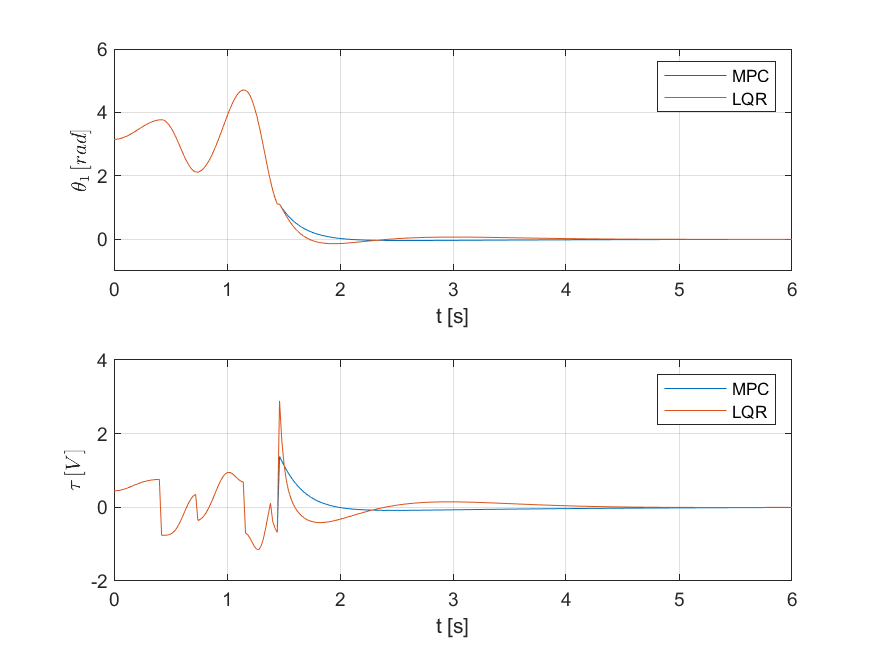
\includegraphics[width=1.1\linewidth]{images/MPC-LQR_Swing}
	\caption{Combined LQR/Swing-Up and MPC/Swing-up control: simulation}
	\label{combo}
\end{figure}
\newpage
\section{NMPC}
NMPC controller is able to fully control the process by itself. To design such controller we use freely availabe \textit{MATMPC} toolbox, which could be downloaded from \textit{https://github.com/chenyutao36/MATMPC}. Also additional software is required:
\begin{itemize}
	\item \textbf{CasAdi} - the state-of-the-art automatic/algorithmic differentiation toolbox.
	\item \textbf{MinGW-w64 C/C++ Compiler} - algorithmic routines are compiled
	into MEX functions using this compiler.
\end{itemize}
As we have all the toolboxes, we use nonlinear model of the process \ref{nonlinmodel} and weight matrices $Q_x$ and $Q_u$, which are designed as:
\begin{equation}
	Q_x = \begin{bmatrix}
	1&0&0&0\\
	0&0.1&0&0\\
	0&0&2&0\\
	0&0&0&0.1
	\end{bmatrix} \quad Q_u = 0.1
\end{equation}
\newpage
\begin{figure}[H]
	\centering
	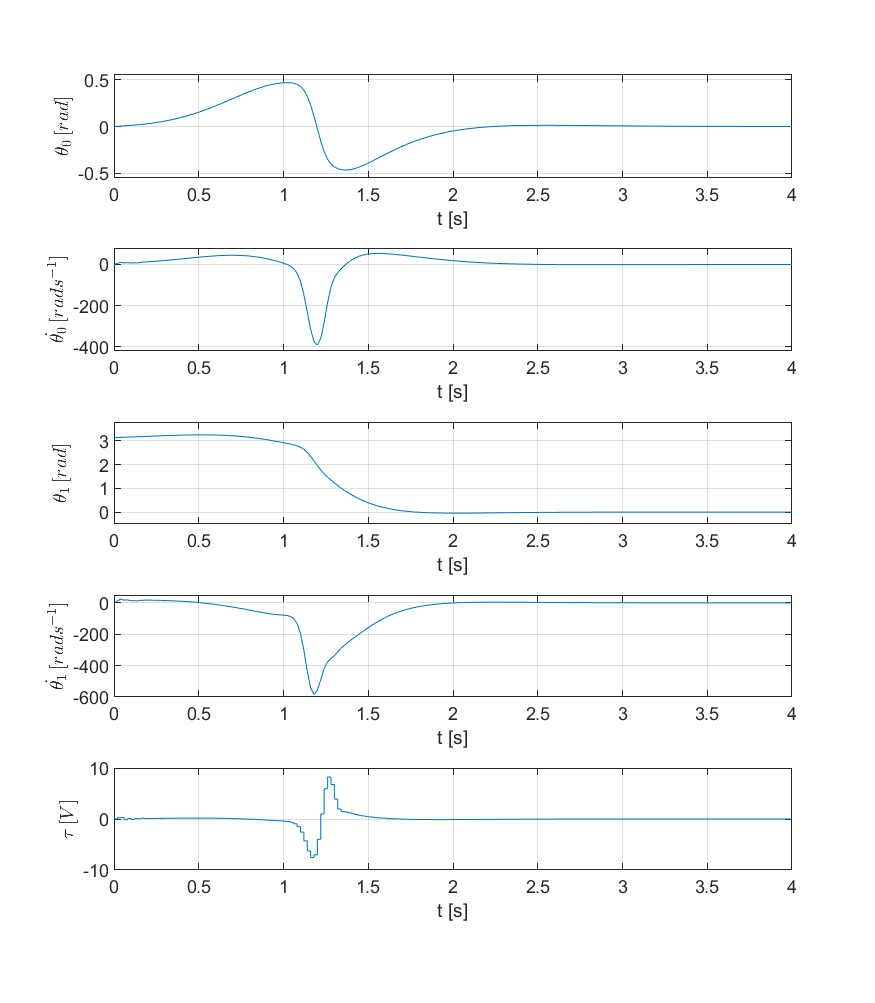
\includegraphics[width=1.1\linewidth]{images/NMPC}
	\caption{NMPC control: simulation}
	\label{NMPC}
\end{figure}